\begin{figure}[!t]
\centering
\resizebox{\columnwidth}{!}{%
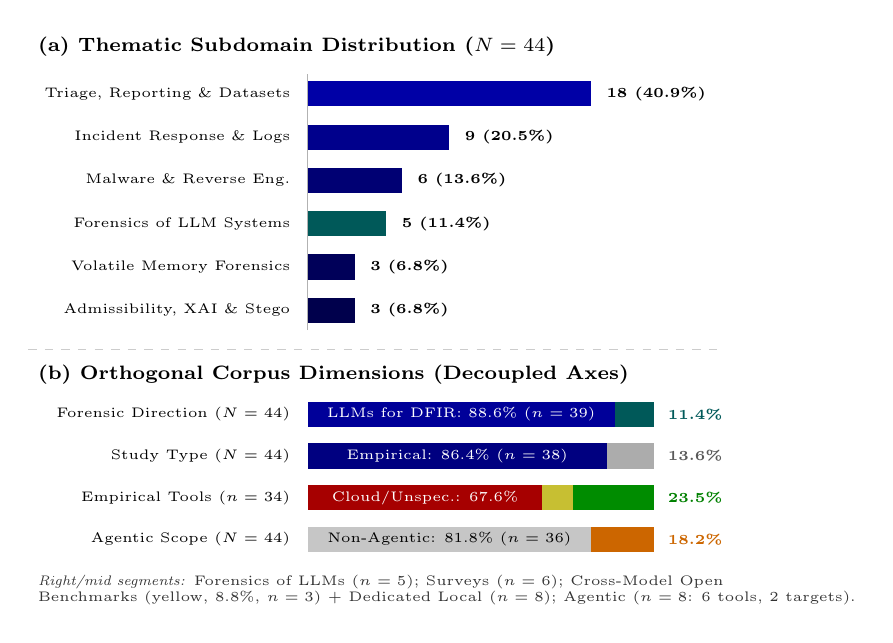
\begin{tikzpicture}[font=\scriptsize]
  % Panel A: Six Operational Subdomains (N=44)
  \node[anchor=west, font=\scriptsize\bfseries] at (0,5.25) {(a) Thematic Subdomain Distribution ($N=44$)};

  % Scale: 18 studies = 3.6 cm -> x = n * 0.20
  \foreach \y/\lbl/\n/\pct/\col in {
    4.65/{Triage, Reporting \& Datasets}/18/{40.9\%}/blue!65!black,
    4.10/{Incident Response \& Logs}/9/{20.5\%}/blue!55!black,
    3.55/{Malware \& Reverse Eng.}/6/{13.6\%}/blue!45!black,
    3.00/{Forensics of LLM Systems}/5/{11.4\%}/teal!70!black,
    2.45/{Volatile Memory Forensics}/3/{6.8\%}/blue!35!black,
    1.90/{Admissibility, XAI \& Stego}/3/{6.8\%}/blue!30!black%
  } {
    \node[anchor=east, font=\tiny] at (3.45,\y) {\lbl};
    \fill[\col] (3.55,\y-0.16) rectangle ({3.55+\n*0.20},\y+0.16);
    \node[anchor=west, font=\tiny\bfseries] at ({3.62+\n*0.20},\y) {\n\ (\pct)};
  }
  \draw[gray!60] (3.55,1.65) -- (3.55,4.90);

  % Divider
  \draw[gray!40, dashed] (0,1.40) -- (8.85,1.40);

  % Panel B: Orthogonal Structural Indicators (100% stacked horizontal bars, width = 4.4cm)
  \node[anchor=west, font=\scriptsize\bfseries] at (0,1.08) {(b) Orthogonal Corpus Dimensions (Decoupled Axes)};

  % Row 1: Forensic Direction (N=44): 39 (88.6%) vs 5 (11.4%)
  \node[anchor=east, font=\tiny] at (3.45,0.58) {Forensic Direction ($N=44$)};
  \fill[blue!60!black] (3.55,0.42) rectangle ({3.55+4.4*0.886},0.74);
  \fill[teal!70!black] ({3.55+4.4*0.886},0.42) rectangle ({3.55+4.4},0.74);
  \node[white, font=\tiny] at (5.50,0.58) {LLMs for DFIR: 88.6\% ($n=39$)};
  \node[anchor=west, font=\tiny\bfseries, text=teal!70!black] at (8.00,0.58) {11.4\%};

  % Row 2: Study Type (N=44): 38 (86.4%) vs 6 (13.6%)
  \node[anchor=east, font=\tiny] at (3.45,0.05) {Study Type ($N=44$)};
  \fill[blue!50!black] (3.55,-0.11) rectangle ({3.55+4.4*0.864},0.21);
  \fill[gray!65] ({3.55+4.4*0.864},-0.11) rectangle ({3.55+4.4},0.21);
  \node[white, font=\tiny] at (5.45,0.05) {Empirical: 86.4\% ($n=38$)};
  \node[anchor=west, font=\tiny\bfseries, text=gray!70!black] at (8.00,0.05) {13.6\%};

  % Row 3: Empirical DFIR Tools (n=34): Cloud/Unspec 23 (67.6%) + Cross-Model Open 3 (8.8%) + Dedicated Local 8 (23.5%)
  \node[anchor=east, font=\tiny] at (3.45,-0.48) {Empirical Tools ($n=34$)};
  \fill[red!65!black] (3.55,-0.64) rectangle ({3.55+4.4*0.676},-0.32);
  \fill[yellow!75!black] ({3.55+4.4*0.676},-0.64) rectangle ({3.55+4.4*0.765},-0.32);
  \fill[green!55!black] ({3.55+4.4*0.765},-0.64) rectangle ({3.55+4.4},-0.32);
  \node[white, font=\tiny] at (5.04,-0.48) {Cloud/Unspec.: 67.6\%};
  \node[anchor=west, font=\tiny\bfseries, text=green!50!black] at (8.00,-0.48) {23.5\%};

  % Row 4: Orchestration (N=44): Non-Agentic 36 (81.8%) vs Agentic 8 (18.2%)
  \node[anchor=east, font=\tiny] at (3.45,-1.01) {Agentic Scope ($N=44$)};
  \fill[gray!45] (3.55,-1.17) rectangle ({3.55+4.4*0.818},-0.85);
  \fill[orange!80!black] ({3.55+4.4*0.818},-1.17) rectangle ({3.55+4.4},-0.85);
  \node[black, font=\tiny] at (5.35,-1.01) {Non-Agentic: 81.8\% ($n=36$)};
  \node[anchor=west, font=\tiny\bfseries, text=orange!80!black] at (8.00,-1.01) {18.2\%};

  % Compact two-line legend for right-hand & middle segments
  \node[anchor=west, font=\tiny, text=black!80, align=left] at (0,-1.65) {\textit{Right/mid segments:} Forensics of LLMs ($n=5$); Surveys ($n=6$); Cross-Model Open\\Benchmarks (yellow, 8.8\%, $n=3$) + Dedicated Local ($n=8$); Agentic ($n=8$: 6 tools, 2 targets).};
\end{tikzpicture}%
}
\caption{Thematic subdomain ranking and decoupled orthogonal structural indicators across the validated corpus ($N=44$), verified via Crossref and OpenAlex (40/44 abstracts/full texts). Deployment locality is evaluated strictly over empirical LLM-for-DFIR tool studies ($n=34$).}
\label{fig:subdomain_matrix}
\end{figure}
